\documentclass[a4paper,report,headsepline]{scrreprt} 

\usepackage{xcolor} 
\usepackage{graphicx}
\usepackage[german]{babel}
\usepackage[utf8]{inputenc}
\usepackage[T1]{fontenc}
\usepackage{ae}
\usepackage{comment}
\usepackage{pdfpages}



\usepackage[automark]{scrlayer-scrpage} 

% headsepline=Dicke:Länge (jeweils optional, die Dicke ist auf 0.4pt voreingestellt)
\KOMAoptions{headsepline=0.5pt} 
\addtokomafont{headsepline}{\color{black}}

\begin{document}


\title{ \begin{Huge}
\textbf{Projektdokumentation}
\end{Huge} \\  \dq Learning Spaces\dq}
\author{Anika Balke (3716066),\\ Daniel Hartmann (369654),\\ Lisa Peter (3682080), \\ Maximilian Hartwich (3730735),\\ Yuliya Karyabochkina (3671623)}
%\date{} %%Wenn kommentiert, wird das aktuelle Datum verwendet.

\maketitle


\tableofcontents
\clearpage



\chapter{Meeting Protokolle}
\underline{{\large Mittwoch, 06.05.2020 Beginn: 10:00 Uhr Ende 10:30 Uhr}}  \\
\textit{Teilnehmer: Lisa Peter, Anika Balke, Maximilian Hartwich, Daniel Hartmann, Yuliya Karyabochkina}

 \begin{itemize}
  \item Allgemeine Besprechung des Vorgehens bei dem Projekt, grobe Zeitplanung der nächsten Wochen
 \item Analyse des Lastenheftes
 \item Verteilung der Aufgaben
 
 \begin{itemize}
 \item Daniel: Festlegung als Product Owner
 \item Anika, Lisa und Yuliya: Erstellung des Pflichtenheftes
 \item Maximilian: Erstellung des UML-Diagrammes sowie der Aktivitätendiagramme
 \item Yuliya: Erstellung des Use-Case- sowie des Anwendungsfalldiagrammes
 \item Daniel: Erste Schritte der Codierung (ausschließlich bekannte Musskriterien des Lastenheftes)
 
\end{itemize} 
\end{itemize}  
 \underline{{\large Mittwoch, 13.05.2020 Beginn: 20:00 Uhr Ende: 20:30 Uhr}}  \\
\textit{Teilnehmer: Lisa Peter, Anika Balke, Maximilian Hartwich, Daniel Hartmann}

\begin{itemize}
 \item Absprache der bisherigen Ergebnisse
\item Sammlung von Fragen für Termin am nächsten Tag mit Herrn Schmidt:
\begin{itemize}
 \item Nur eine Buchung pro Woche: Ist nach Stornierung eine Buchung für die gleiche Woche möglich oder erst für die kommende Woche?
\item Wie detailliert sollen die Aktivitäten im Aktivitätsdiagramm beschrieben werden?
\item Wie detailliert sollen die Aktivitäten im Use-Case Diagramm beschrieben werden?
\item Welche Räume sollen installiert werden? (Größe, Lage, usw.)
\item Ist ein genauer Platz in den Räumen buchbar oder nur allgemein ein Platz?
\item Blocklänge: mit (Mittags-) Pause?
\item Dürfen die Belegungen der Räume öffentlich einsehbar sein oder nur für eingeloggte User? 

\end{itemize} 
\end{itemize}  
 \underline{{\large Donnerstag, 14.05.2020 Beginn: 9:00 Uhr Ende: 9:45 Uhr}}  \\
\textit{Teilnehmer: Lisa Peter, Anika Balke, Maximilian Hartwich, Daniel Hartmann, Yuliya Karyabochkina, Michael B. Schmidt}

\begin{itemize}
\item Allgemeine Besprechung des Projektstatus
\item Kundengespräch mit folgenden Festlegungen und Inhalten: 
\begin{itemize}
\item Ansicht der Belegungen maximal eine Woche im Voraus
\item Jeden Vorgang mit Hilfe eines Aktivitätendiagrammes beschreiben
\item Größe der Räume soll von der Gruppe definiert werden
\item Raumbuchungen dürfen nur für eingeloggte User sichtbar sein
\item Bestätigungsemail bei erfolgreicher Raumbuchung als Wunschkriterium

\end{itemize} 
\end{itemize}
 \underline{{\large Mittwoch, 20.05.2020, Beginn: 10:00 Uhr Ende: 10:45 Uhr}}  \\
\textit{Teilnehmer: Lisa Peter, Anika Balke, Maximilian Hartwich, Daniel Hartmann, Yuliya Karyabochkina}

\begin{itemize}
\item Gemeinsame Besprechung:

\begin{itemize}
\item Bisher angefertigter Diagramme
\item Aktueller Stand des Pflichtenheftes
\end{itemize}

\item Klärung verschiedener Fragen zu den einzelnen Funktionen für die Erstellung des Pflichtenheftes
\item Besprechung des aktuellen Programmierstandes und Festlegung des Programmierstandes bis zum nächsten Kundentermin mit Herrn Schmidt:
\begin{itemize}
\item Layout der Startseite
\item Buchungsübersicht
\item Layout bei dem Buchungsvorgang

\end{itemize}
\end{itemize} 
 \underline{{\large Dienstag, 26.05.2020, Beginn: 14:15 Uhr, Ende 15:15 Uhr}}  \\
\textit{Teilnehmer: Lisa Peter, Anika Balke, Maximilian Hartwich, Daniel Hartmann, Yuliya Karyabochkina, Michael B. Schmidt}

\begin{itemize}
\item Allgemeine Besprechung des Projektstatus
\item Besprechung verschiedener Funktionen
\item Weitere Muss- und Wunschkriterien mit Herrn Schmidt abgesprochen
\item Diverse Rahmenbedingungen abgeklärt
\item Abgleich der Diagramme mit Herrn Schmidt
\item Präsentation einer bisherigen Layoutsskizze 

\end{itemize}
 \underline{{\large 04.06.2020 Beginn: 19:50 Uhr Ende: 21:30 Uhr}}  \\
\textit{Teilnehmer: Lisa Peter, Anika Balke, Maximilian Hartwich, Daniel Hartmann, Yuliya Karyabochkina}

\begin{itemize}
\item Durchsprache der bisherigen Ergebnisse aller Gruppenmitglieder
\item Besprechung der Ergebnisse im Pflichtenheft, Einfügen der erforderlichen Diagramme (UML-Diagramm, Use-Case Diagramm, Aktivitätendiagramme)
\item Anpassung und Überarbeitung des Pflichtenheftes

\end{itemize}

 
\section{Scrum-Meetings} 
 \underline{{\large SCRUM-Meeting Nr. 1, Mittwoch, 10.06.2020, Beginn: 10:00 Uhr Ende 10:30 Uhr}}  \\
\textit{Teilnehmer: Lisa Peter, Anika Balke, Maximilian Hartwich, Daniel Hartmann, Yuliya Karyabochkina}

\begin{itemize}
\item Festlegen der Sprintdauer auf eine Woche
\item Verteilung der eingehenden Aufgaben:
\begin{itemize}
\item Nach Feedback des Kundens (26.05.2020) detailliertere Codierung der bisherigen Benutzeroberfläche (Startseite, Buchungsübersicht, Buchungsvorgang) --> Daniel (2 Sprints)
\item Erstellung der Datei für die Dokumentation und Bereitstellung auf GitHub $\rightarrow$ Lisa \& Anika (1 Sprint)
\item Planung der Implementierung der Funktionen in die Seite (1 Sprint) --> Maximilian \& Yuliya 
\end{itemize}
\end{itemize}
 \underline{{\large SCRUM-Meeting Nr. 2, Mittwoch, 17.06.2020, Beginn: 10:30 Uhr Ende 11:15 Uhr}}  \\
\textit{Teilnehmer: Lisa Peter, Anika Balke, Maximilian Hartwich, Daniel Hartmann, Yuliya Karyabochkina}
      

\begin{itemize}
\item Durchsprache der bisherigen Ergebnisse
\item Klärung offener Fragen (Probleme bei der Dokumentation auf GitHub)
\item Verteilung der Aufgaben für die kommende Woche
\begin{itemize}
\item Anmeldung programmieren: Eingabefelder für Benutzername und Passwort, Login-Button, Design der Startseite --> Daniel (1 Sprint übrig)
\item Coding der Raumübersicht: Ansicht verschiedener Räume mit Infotext über jeweiligen Raum --> Yuliya \& Maximilian (2 Sprints)
\item Problembehebung auf GitHub --> Lisa \& Anika (1 Sprint)

\end{itemize}
\end{itemize}
 \underline{{\large SCRUM-Meeting Nr. 3, Mittwoch, 24.06.2020, Beginn: 10:30 Uhr Ende 11:15 Uhr}}  \\
\textit{Teilnehmer: Lisa Peter, Anika Balke, Maximilian Hartwich, Daniel Hartmann, Yuliya Karyabochkina}      

\begin{itemize}
\item Durchsprache aktueller Stand, Probleme bei der Programmierung: es wurde festgestellt, dass kleinere Pakete verteilt werden müssen (Statt „Codierung Startseite“ eher „Codierung Login-Button“ und „Codierung Eingabefelder“
\item Aufgabenverteilung für die nächste Woche:
\begin{itemize}
\item Coding der zur Verfügung stehenden Zeitslots --> Anika (1 Sprint)
\item Coding: maximal eine Buchung pro Woche möglich --> Lisa (1 Sprint)
\item Coding der Reservierungsübersicht: Ansicht eines jeweiligen Raumes mit allen notwendigen Angaben (Datum, Raum, Zeitblock), Button zur Stornierung der angezeigten Reservierung --> Maximilian (2 Sprints)
\item PopUp zur Bestätigung der Reservierung --> Yuliya (1 Sprint)

\end{itemize}
\end{itemize}
 \underline{{\large SCRUM-Meeting Nr. 4, Mittwoch, 01.07.2020, Beginn: 17:45 Uhr Ende 18:15 Uhr}}  \\
\textit{Teilnehmer: Lisa Peter, Anika Balke, Maximilian Hartwich, Daniel Hartmann, Yuliya Karyabochkina} 

\begin{itemize}
\item Rücksprache über aktuelle Arbeitspakete (erledigt, Probleme, Verlängerung notwendig oder Sonstiges)
\item Aufgabenverteilung für die nächste Woche:
\begin{itemize}
\item PopUp bei belegtem Space und User --> Anika (1 Sprint)
\item Überbuchungsfunktion, wenn User = Mitarbeiter --> Daniel (1 Sprint)
\item Eigene Raumbuchung anzeigen lassen --> Yuliya (1 Sprint)
\item Stornierungsfunktion --> Maximilian (1 Sprint)
\item Anzeigeoption freier Räume über Suchfunktion --> Daniel (1 Sprint)
\item Anzeige zur Verfügung stehender Funktionen --> Lisa (1 Sprint)

\end{itemize}
\end{itemize}
 \underline{{\large SCRUM-Meeting Nr. 5, Mittwoch, 08.07.2020, Beginn: 12:30 Uhr Ende 13:30 Uhr}}  \\
\textit{Teilnehmer: Lisa Peter, Anika Balke, Maximilian Hartwich, Daniel Hartmann, Yuliya Karyabochkina} 

\begin{itemize}
\item Allgemeine Besprechung des Projektstatus
\item Rücksprache über aktuelle Arbeitspakete (erledigt, Probleme, Verlängerung notwendig oder Sonstiges)
\item Aufgabenverteilung für die nächste Woche:
\begin{itemize}
\item Hilfe über Kontaktformular anfragen --> Maximilian (1 Sprint)
\item E-Mail zur Benachrichtigung bei Buchung, Stornierung --> Daniel (1 Sprint)
\item Internationalisierung des Systems (System in englischer Sprache) 
--> Yuliya (1 Sprint)
\item Abschlussdokumentation der Projektarbeit --> Anika \& Lisa

\end{itemize}
\end{itemize}
 \underline{{\large SCRUM-Meeting Nr. 6, Mittwoch, 15.07.2020, Beginn: 10:30 Uhr Ende 11:15 Uhr}}  \\
\textit{Teilnehmer: Lisa Peter, Anika Balke, Maximilian Hartwich, Daniel Hartmann, Yuliya Karyabochkina}

\begin{itemize}
\item Rücksprache über aktuelle Arbeitspakete (erledigt, Probleme, Verlängerung notwendig oder Sonstiges)
\item Sammeln von Ideen für mögliche weitere „Kann“-Funktionen und Aufteilung einiger auf die nächste Woche
\begin{itemize}
\item Anonyme Anfrage belegter Räume --> Daniel (1 Sprint)
\item Hinweis, bei falscher Kennworteingabe beim Login --> Maximilian (1 Sprint)
\item Kalenderfunktion --> Yuliya (1 Sprint)
\item Anzeige personenbezogener Daten --> Daniel (1 Sprint)
\item Abschlussdokumentation in Latex --> Lisa \& Anika (Running ToDo bis zum Projektabschluss)

\end{itemize}
\end{itemize}
 \underline{{\large SCRUM-Meeting Nr. 7, Mittwoch, 22.07.2020, Beginn: 10:30 Uhr Ende 11:15 Uhr}}  \\
\textit{Teilnehmer: Lisa Peter, Anika Balke, Maximilian Hartwich, Daniel Hartmann, Yuliya Karyabochkina}

\begin{itemize}
\item Rücksprache über aktuelle Arbeitspakete (erledigt, Probleme, Verlängerung notwendig oder Sonstiges)
\item Aufgabenverteilung für die nächste Woche:
\begin{itemize}
\item Änderung des eigenen Passworts / der E-Mail Adresse --> Daniel (1 Sprint)
\item Logout --> Yuliya (1 Sprint)
\item Anlegen, Editieren und Löschen von Benutzerkonten durch den Admin --> Maximilian (1 Sprint)
\item Anlegen und Editieren von Space-bezogenen Daten ausschließlich durch den Admin --> Maximilian (1 Sprint)
\item Anlegen, Editieren und Löschen der Ressourcen der Learning Spaces --> Daniel (2 Sprints)
\item Abschlussdokumentation in Latex --> Lisa \& Anika (Running ToDo bis zum Projektabschluss)

\end{itemize}
\end{itemize}
 \underline{{\large SCRUM-Meeting Nr. 8, Mittwoch, 29.07.2020, Beginn: 10:15 Uhr Ende 11:45 Uhr}}  \\
\textit{Teilnehmer: Lisa Peter, Anika Balke, Maximilian Hartwich, Daniel Hartmann, Yuliya Karyabochkina}
\begin{itemize}
\item Allgemeine Besprechung des Projektstatus
\item Rücksprache über aktuelle Arbeitspakete (erledigt, Probleme, Verlängerung notwendig oder Sonstiges)
\item Sammeln erster Ideen für mögliche Testszenarien --> alle
\item Einfügen fehlender Kommentare im Quelltext --> Daniel \& Maximilian (Running ToDo bis zum Projektabschluss)
\item Fertigstellung der Programmierung, damit ab nächster Woche Testszenarien durchgeführt werden können und Fehlermeldungen behoben werden können. --> Daniel \& Maximilian (Running ToDo bis zum Projektabschluss)
\item Aufgabenverteilung für die nächste Woche:
\begin{itemize}
\item Abschlussdokumentation der Projektarbeit --> Anika \& Lisa
\item Beschreibung der API Endpunkte --> Daniel (2 Sprints)

\end{itemize}
\end{itemize}
 \underline{{\large SCRUM-Meeting Nr. . 9, Mittwoch, 05.08.2020, Beginn: 10:00 Uhr Ende 11:30 Uhr}}  \\
\textit{Teilnehmer: Lisa Peter, Anika Balke, Maximilian Hartwich, Daniel Hartmann, Yuliya Karyabochkina}
\begin{itemize}
\item Durchsprache des aktuellen Standes des Projektes
\item Besprechung des Zeitplans / noch durchzuführender Aufgaben bis Ende August
\item Durchführung eines ersten Testszenarios - Student: 
\begin{itemize}
\item Anzeige aller möglicher zu buchender Learning Spaces
\item Buchung eines Learning Spaces zu einem bestimmten Block
\item Anzeige aller persönlichen getätigten Buchungen
\item Stornierung der getätigten Buchung
\item Über Kontaktformular automatische Kontaktaufnahme bei Nachfragen / Komplikationen
\end{itemize}
\item Aufgabenverteilung für die nächste Woche:
\begin{itemize}
\item Abschlussdokumentation der Projektarbeit --> Anika \& Lisa
\item Beschreibung der API Endpunkte --> Daniel (1 Sprint übrig)
\item Beschreibung des durchgeführten Tests --> Anika \& Lisa (1Sprint)
\item Einfügen fehlender Kommentare im Quelltext --> Daniel \& Maximilian (Running ToDo bis zum Projektabschluss)
\item Fertigstellung der Programmierung, damit ab nächster Woche Testszenarien durchgeführt werden können und Fehlermeldungen behoben werden können. --> Daniel \& Maximilian (Running ToDo bis zum Projektabschluss)

\end{itemize}
\end{itemize}
 \underline{{\large SCRUM-Meeting Nr. 10, Mittwoch, 12.08.2020, Beginn: 09:00 Uhr Ende 10:45 Uhr}}  \\
\textit{Teilnehmer: Lisa Peter, Anika Balke, Maximilian Hartwich, Daniel Hartmann, Yuliya Karyabochkina}
\begin{itemize}
\item Allgemeine Besprechung des Projektstatus
\item Durchführung eines ersten Testszenarios - Dozent: 
\begin{itemize}
\item Anzeige aller möglicher zu buchender Learning Spaces
\item Buchung eines Learning Spaces zu einem bestimmten Block
\item Anzeige aller persönlichen getätigten Buchungen
\item Stornierung der getätigten Buchung
\item Überbuchung eines bereits belegten Learning Spaces zu einem bestimmten Zeitpunkt
\end{itemize}
\item Aufgabenverteilung für die nächste Woche
\begin{itemize}
\item Abschlussdokumentation der Projektarbeit --> Anika \& Lisa
\item Beschreibung des durchgeführten Tests --> Yuliya (1 Sprint)
\item Durchführung letzter Feinheiten an der Programmierung --> Daniel \& Maximilian (1Sprint)

\end{itemize}
\end{itemize}
\underline{{\large SCRUM-Meeting Nr. 11, Montag, 17.08.2020, Beginn: 14:15 Uhr Ende 15:45 Uhr }} \\
\textit{Teilnehmer: Lisa Peter, Anika Balke, Maximilian Hartwich, Daniel Hartmann, Yuliya Karyabochkina, Michael B. Schmidt }

\begin{itemize}
\item Allgemeine Besprechung des Projektstatus 
\item Durchsprache des aktuellen Standes der Programmierung und Vorführung des Raumbuchungssystems 
\item Abklärung letzter Fragen bezüglich der Abschlussdokumentation der Projektarbeit 
\item Abklärung letzter Fragen bezüglich der Abgabe des Projektes 
\end{itemize}
\underline{{\large SCRUM-Meeting Nr. 12, Mittwoch, 24.08.2020, Beginn: 9:00 Uhr Ende 9:45 Uhr}} \\
\textit{Teilnehmer: Lisa Peter, Anika Balke, Maximilian Hartwich, Daniel Hartmann, Yuliya Karyabochkina}

\begin{itemize}
\item Allgemeine Besprechung des Projektstatus 
\item Durchsprache der letzten zu erledigenden Aufgaben 
\item Abschlussdokumentation der Projektarbeit fertigstellen --> Maximilian, Anika \& Lisa (1 Sprint) 
\item Fortschreibung des Zeitplans mit den erledigten Arbeitspaketen --> Yuliya (1 Sprint) 
\item Finalisierung der Programmierung für die Abgabe des Projektes --> Daniel (1 Sprint) 
\end{itemize}
\underline{{\large SCRUM-Meeting Nr. 13, Freitag, 28.08.2020, Beginn: 15:00 Uhr Ende 16:15 Uhr}} \\
\textit{Teilnehmer: Lisa Peter, Anika Balke, Maximilian Hartwich, Daniel Hartmann, Yuliya Karyabochkina}

\begin{itemize}
\item Allgemeine Besprechung des Projektstatus 
\item Kontrolle aller notwendigen Dinge bezüglich der Projektarbeit 
\item Durchsicht der Abschlussdokumentation 
\item Kontrolle der Github Repo für den Sourcecode und die Doku 
\end{itemize}
     
\chapter{Github Repo}
Der Quellcode und die Dokumentation des Projektes wurden mit der Versionsverwaltungskontrolle GitHub verwaltet und so die Arbeit von allen Mitgliedern des Projektteams zusammengeführt. Nachfolgend sind beide Repositorys aufgeführt.\\
\underline{Dokumentation:} https://github.com/dnhrtmn/IuKDokumentation.git \\
\underline{Projekt:} https://github.com/dnhrtmn/IuK.git
\chapter{Fortschreibung des Zeitplans mit den erledigten Arbeitspaketen}
Um die Realisierung des Projektes möglichst strukturiert und zielorientiert zu gestalten wurde ein Projektzeitplan, der in regelmäßigen Abständen besprochen und angepasst wurde, erstellt. Dieser konkretisiert die einzelnen Projektphasen und Arbeitspakete. \\ 
Zur Umsetzung des Projektes wurden insgesamt 100 Stunden pro Person zur Verfügung gestellt. Vor dem Beginn des Projektes wurde diese Zeit in verschiedene Phasen aufgeteilt, die während des Entwicklungsprozesses durchlaufen werden. Der Abschluss einer Phase stellt jeweils ein Meilenstein des Projektes dar.  
Auf der nachfolgenden Seite 14 ist der Projektzeitplan abgebildet.
\\
In der Spalte „Aufgabe“ wurden die relevanten Aufgaben zur Umsetzung des Projektes eingetragen. In der Spalte „Zuständigkeit“ wurde eingetragen welches Mitglied des Projektteams für die jeweilige Aufgabe zuständig war. Abschließend wurden in der Spalte „Zeitplan“, aufgeteilt nach Kalenderwochen, die relevantesten Projekt-Meilensteine (orange) sowie der vorgesehene Zeitraum zur Bearbeitung der Arbeitsschritte (grün) farblich gekennzeichnet. \\
Der Vollständigkeit halber und zum Abgleich des zu Beginn geplanten und des tatsächlich realisierten Zeitplans ist in folgender Abbildung der zu Beginn festgelegte grobe Zeitplan abzulesen. 
\begin{figure}[h]
    \centering
    \caption{Zeitplan}
    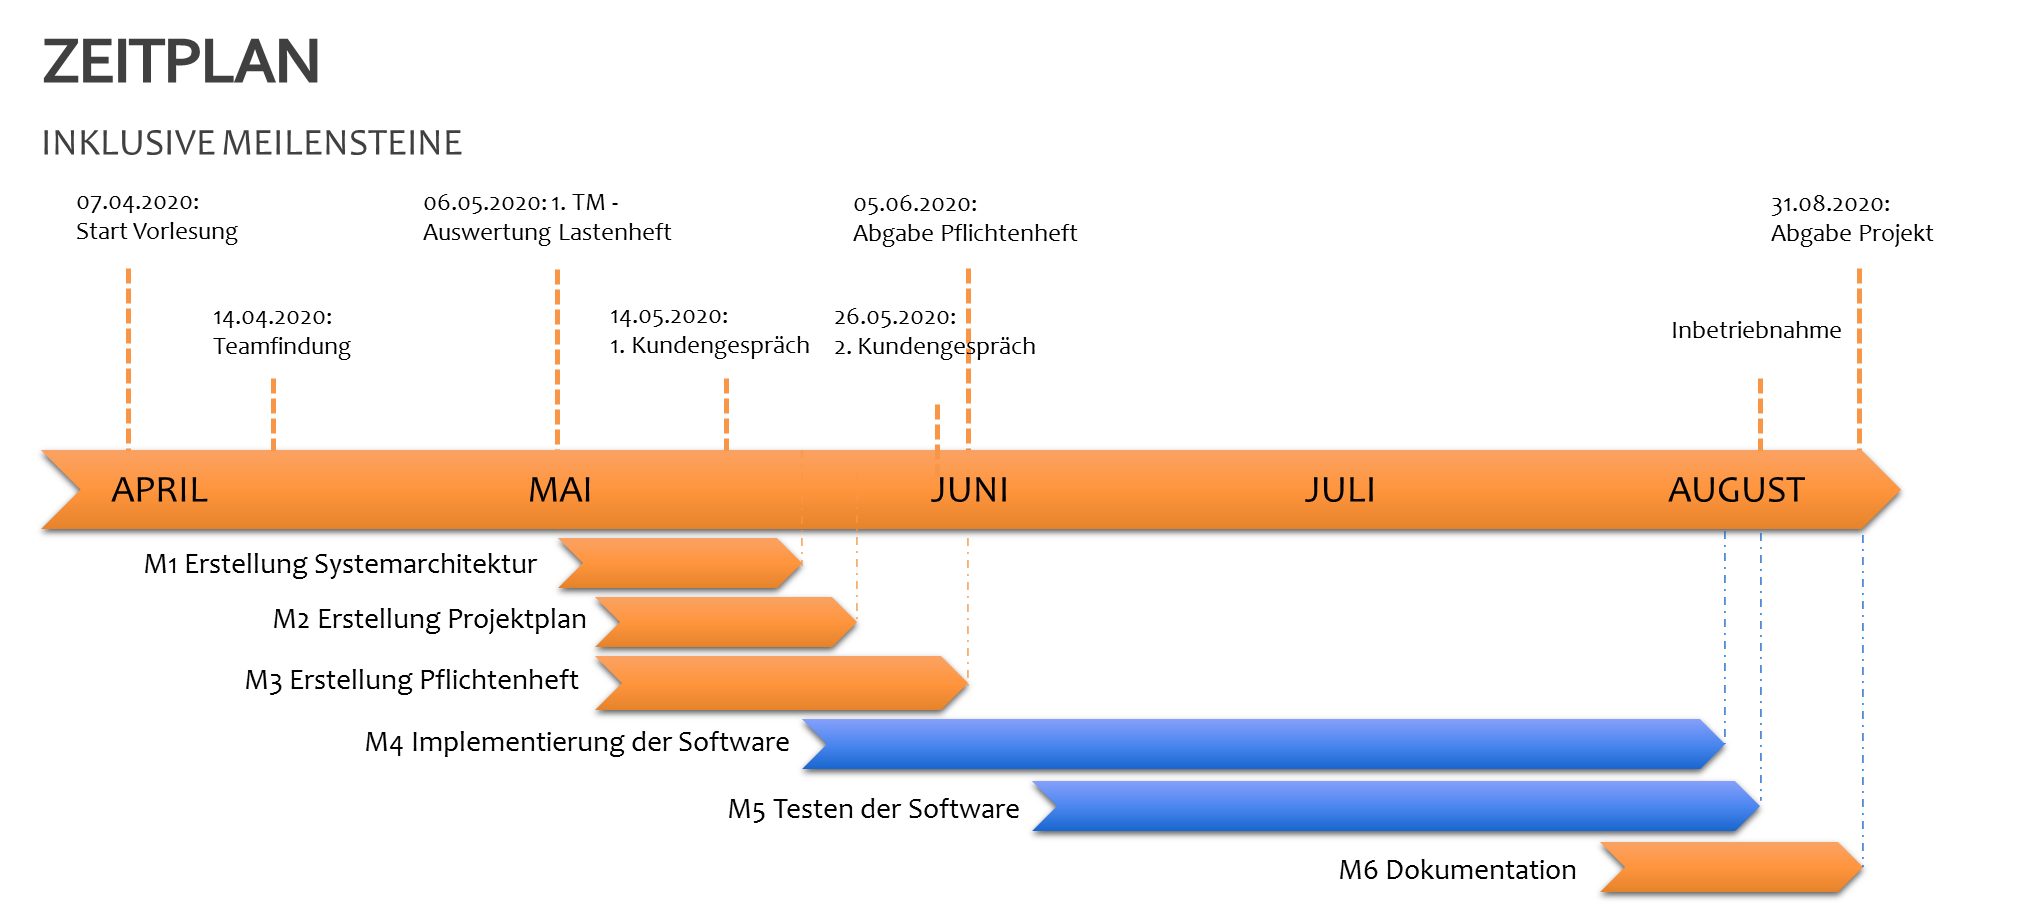
\includegraphics[width=0.8\textwidth]{Zeitplan_2}
    \label{fig:Zeitplan}
\end{figure}

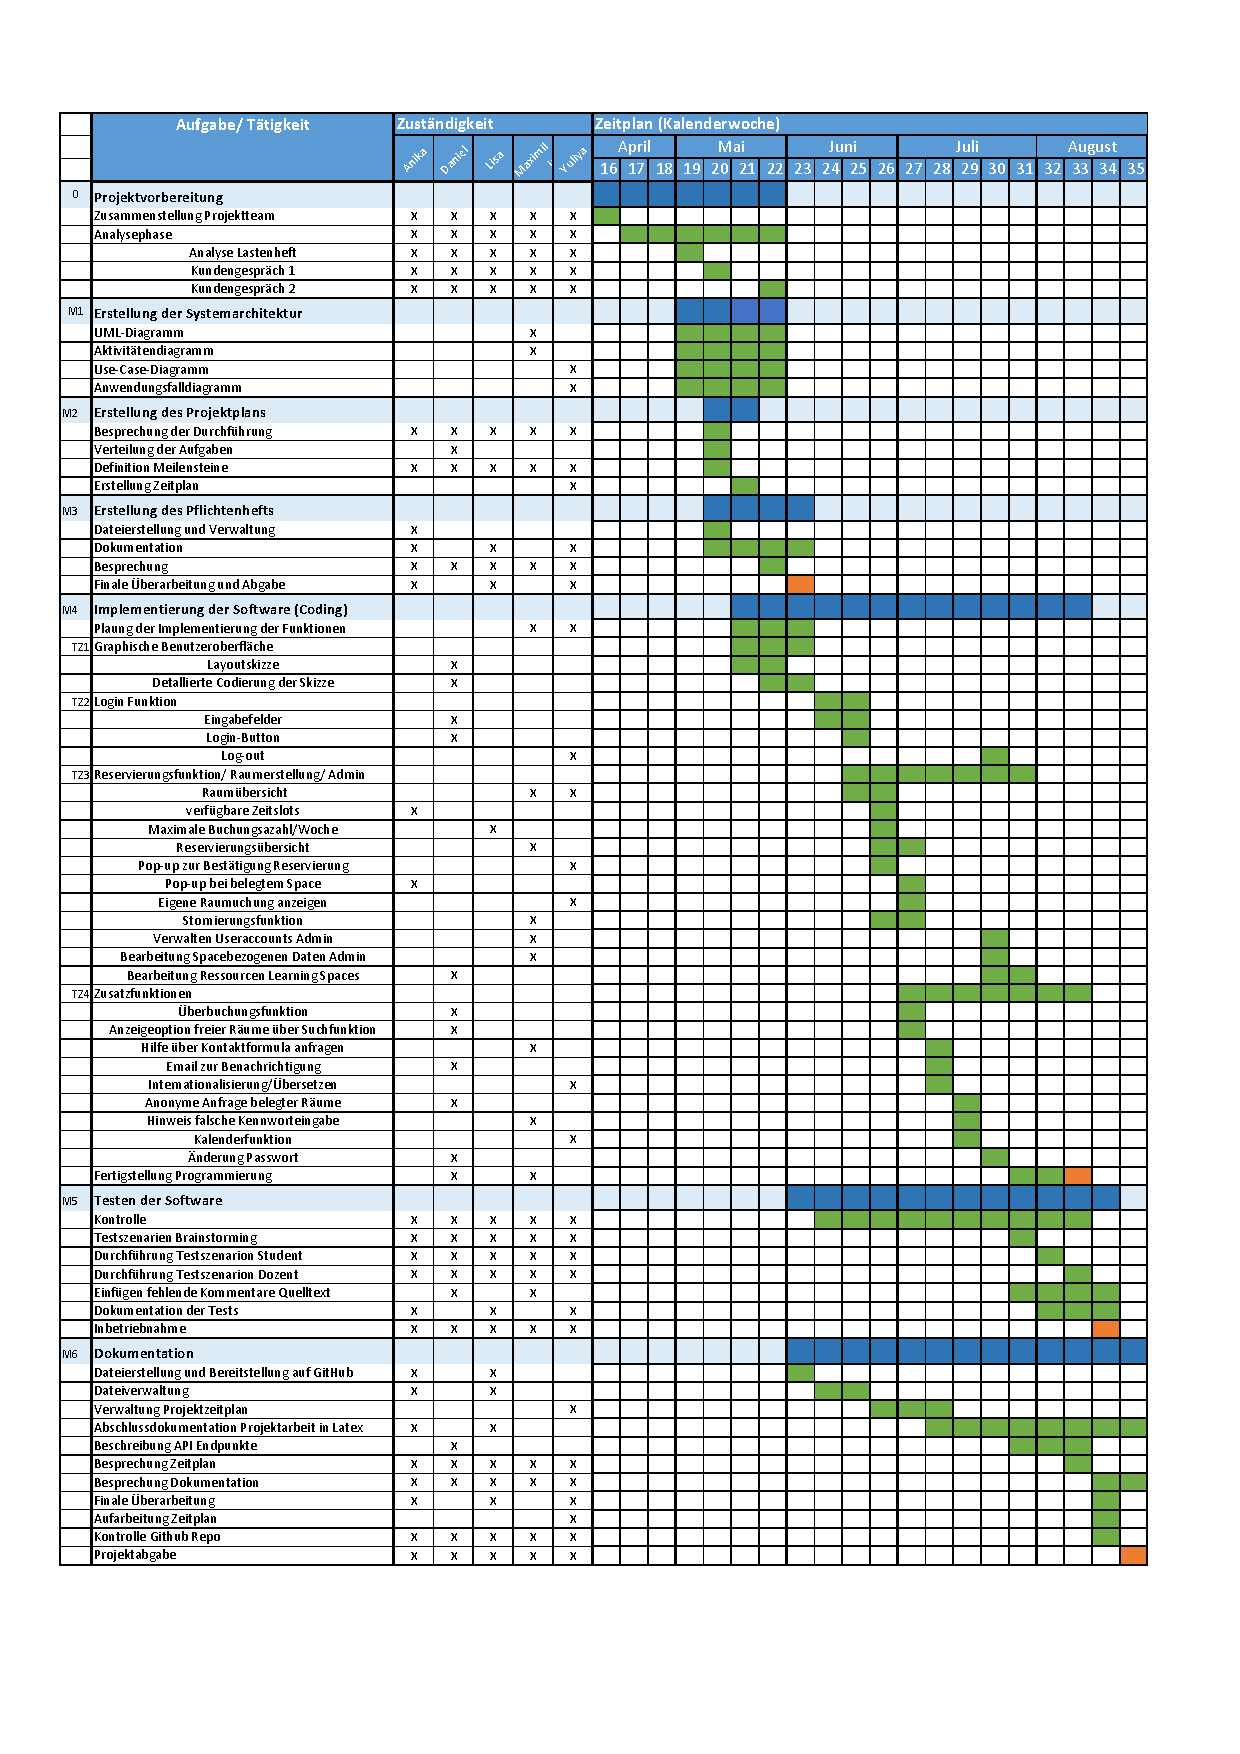
\includepdf[pages=-, pagecommand={\thispagestyle{plain}}]{Projektzeitplan}

\chapter{Produktdokumentation basierend auf dem Pflichtenheft}\label{cha:Produktdokumentation}
\section{Für den Anwender erforderliche Login-Informationen}
Alle Mails, die vom System an den Nutzer gesendet werden sind unter folgendem Link ersichtlich: \textbf{www.Mailtrap.io}. \\
Zum Login bitte mit dem Nutzernamen \dq \textbf{da.hartmann@me.com}\dq{} 
und dazugehörigem Passwort \dq  \textbf{DidPfIuk2020!}\dq{} anmelden.
\section{Grundsätzliche Funktionen inklusive Muss-Kriterien}
Nach dem Öffnen der Seite kann sich der User (Admin, Dozent, Mitarbeiter, Student) über die vorhandenen Eingabeflächen mit der privaten E-Mail-Adresse sowie seinem Kennwort anmelden (F25). Zusätzlich wird ihm über einen Reiter die Option geboten, sich die Seite entweder auf Deutsch oder Englisch anzeigen zu lassen, was die Software gerade für Austauschstudenten benutzerfreundlicher macht (F16). 
\begin{figure}[h]
    \centering
    \caption{Login mit ausgefahrenem Reiter}
    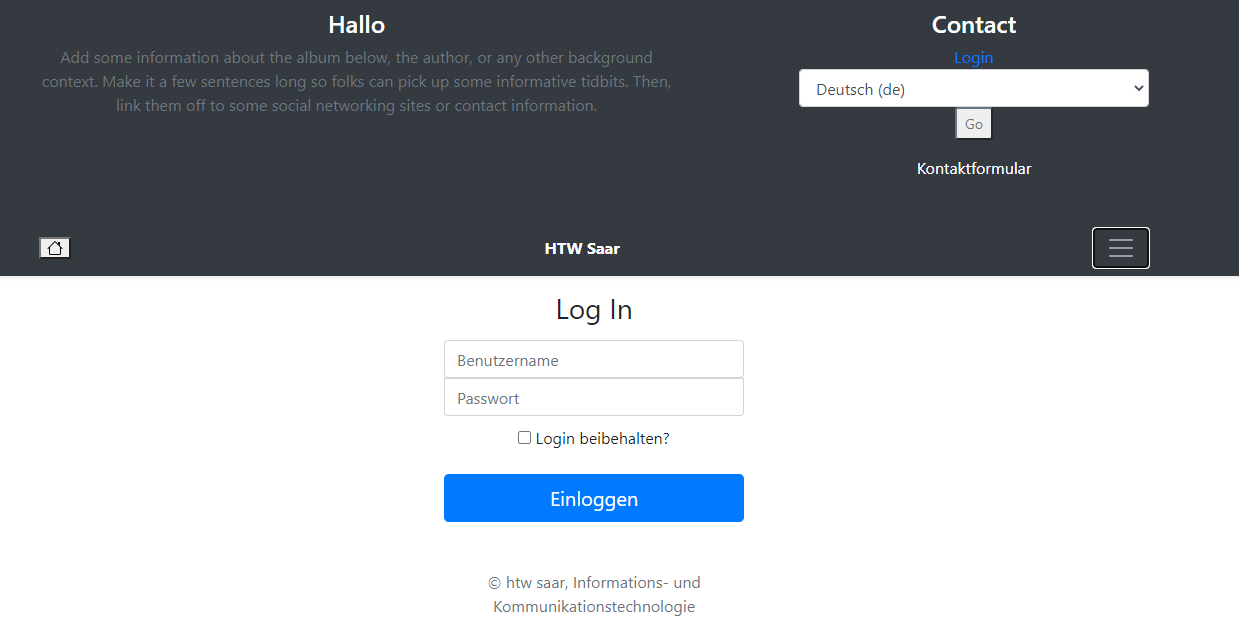
\includegraphics[width=0.8\textwidth]{Login mit ausgefahrenem Reiter}
    \label{fig:Login mit ausgefahrenem Reiter}
\end{figure}
Nach dem erfolgreichen Login befindet sich der User auf der Home-Ansicht. Von dort aus kann er sich zu verschiedenen Seitenansichten navigieren. Über die Raumbelegungsanzeige werden alle vorhandenen Räume/Spaces angezeigt (F10).
\begin{figure}[h]
    \centering
    \caption{Raumanzeige}
    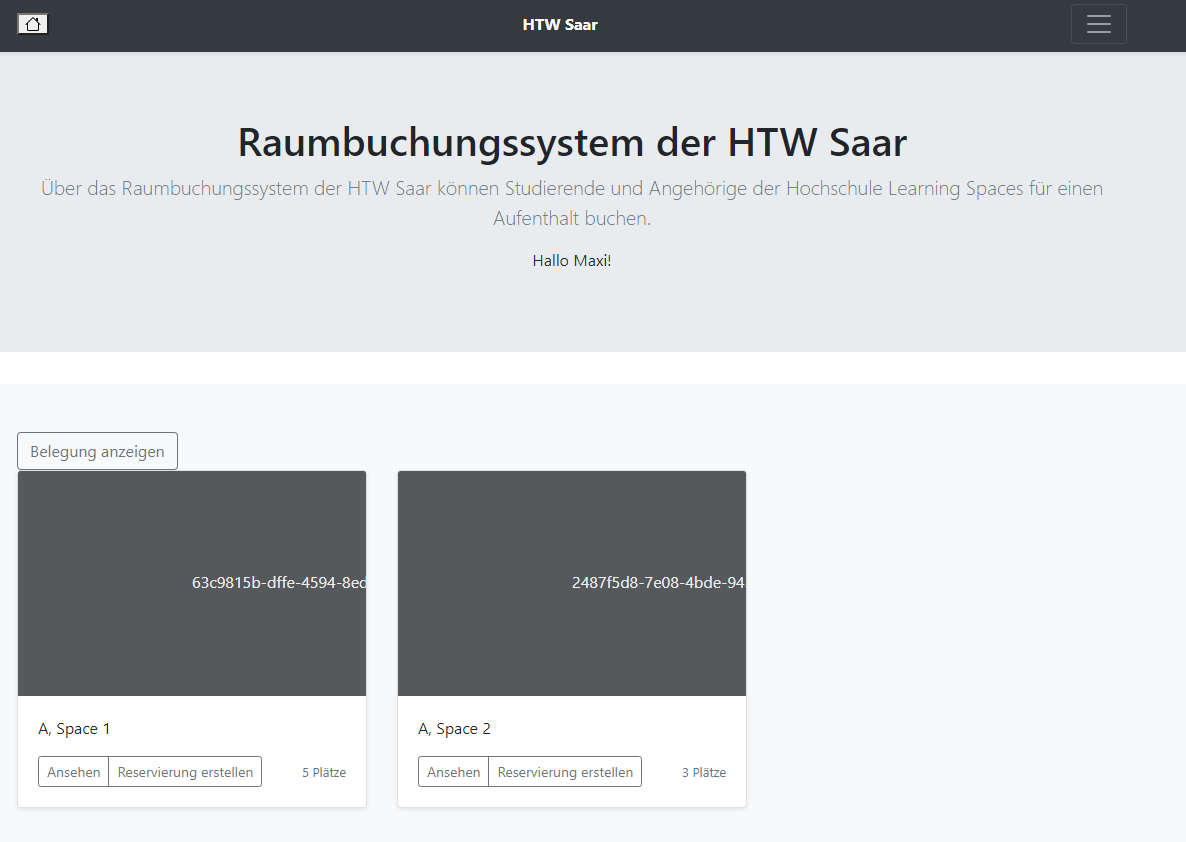
\includegraphics[width=0.8\textwidth]{Raumanzeige}
    \label{fig:Raumanzeige}
\end{figure}
Bei der Auswahl eines Raumes, erscheint eine Wochenanzeige des jeweiligen Raumes mit allen möglichen Blöcken und deren zeitliche Begrenzungen (F12).
\begin{figure}[h]
    \centering
    \caption{Wochenanzeige}
    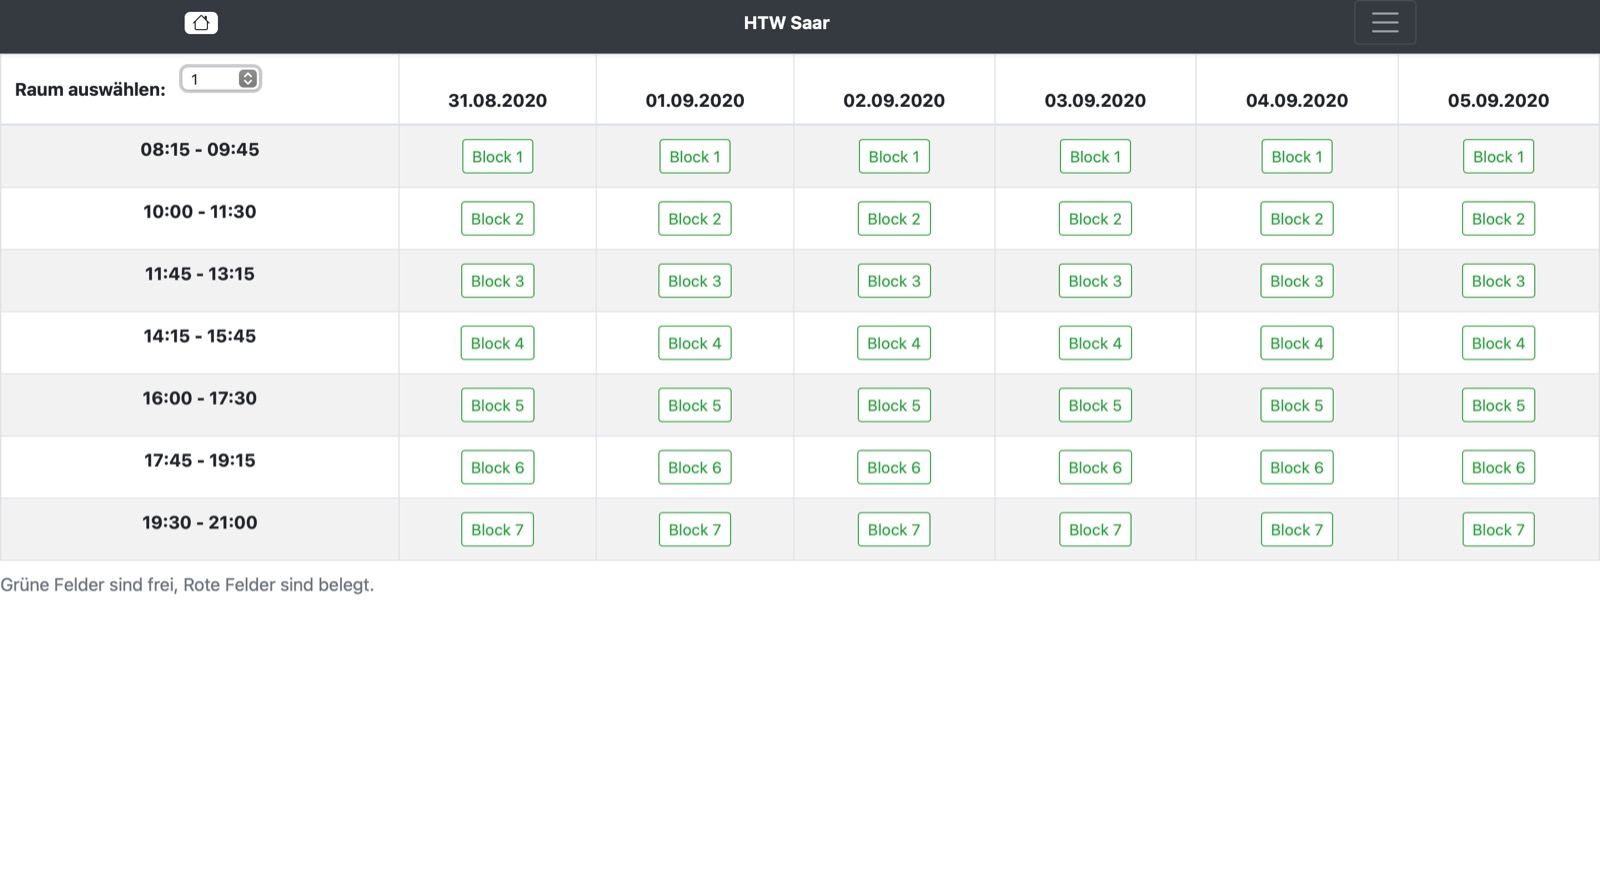
\includegraphics[width=0.8\textwidth]{Wochenanzeige}
    \label{fig:Wochenanzeige}
\end{figure}
\clearpage
Dabei stehen grün hinterlegte Blöcke für ungebuchte/freie und rot hinterlegte für bereits gebuchte/belegte Blöcke. Der User hat die Möglichkeit entweder einen freien Block auszuwählen und diesen über eine Schaltfläche zu buchen (F18) oder einen gebuchten Block, für den er eine Nutzungsanfrage an den jeweiligen User schicken kann (F19).\\
\begin{figure}[h]
    \centering
    \caption{Reservierungsübersicht}
    \includegraphics[width=0.8\textwidth]{Reservierungsübersicht}
    \label{fig:Reservierungsübersicht}
\end{figure}
\begin{figure}[h]
    \centering
    \caption{Buchungsvorgang}
    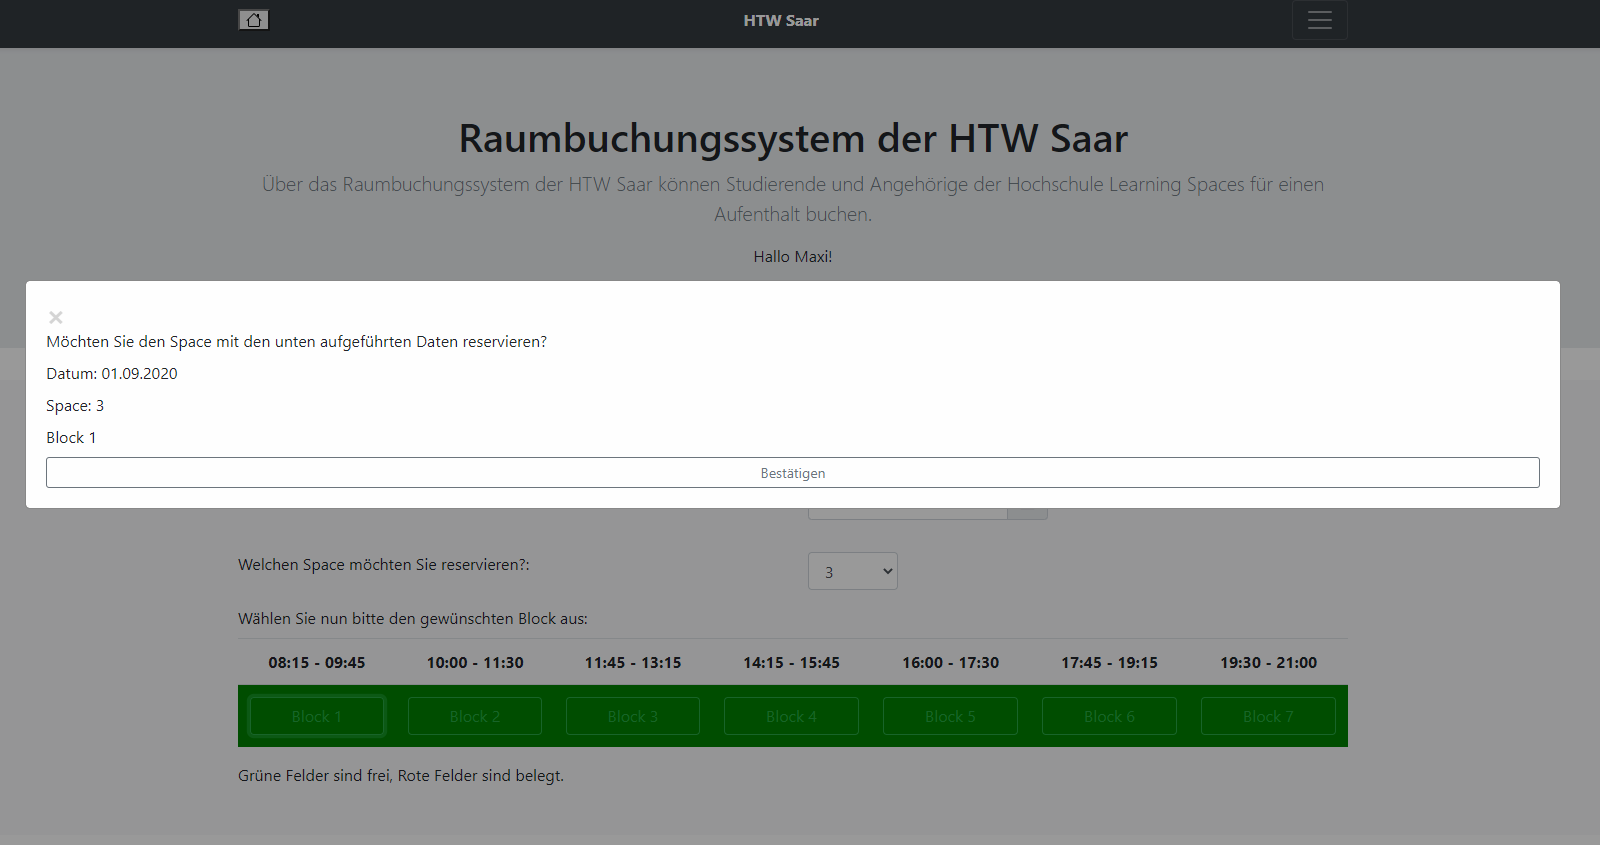
\includegraphics[width=0.8\textwidth]{Buchungsvorgang}
    \label{fig:Buchungsvorgang}
\end{figure}
Im Falle einer freien Buchung erhält der User eine Bestätigungsmail (L11). Dozenten haben zusätzlich das Recht gebuchte Blöcke ohne Zustimmung des anderen Users (Mitarbeiter/Student) zu überbuchen (F20). Auch in diesem Fall wird der User per Mail über die Überbuchung informiert. Sollte der User bemerken, dass er den von ihm gebuchten Termin nicht wahrnehmen kann, kann er diesen in der persönlichen Reservierungsübersicht, in der alle vergangenen und auch bevorstehenden Buchungen gelistet sind (F13/F14), über den „Delete“-Button stornieren (F21).

\begin{figure}[h]
    \centering
    \caption{Stornieren}
    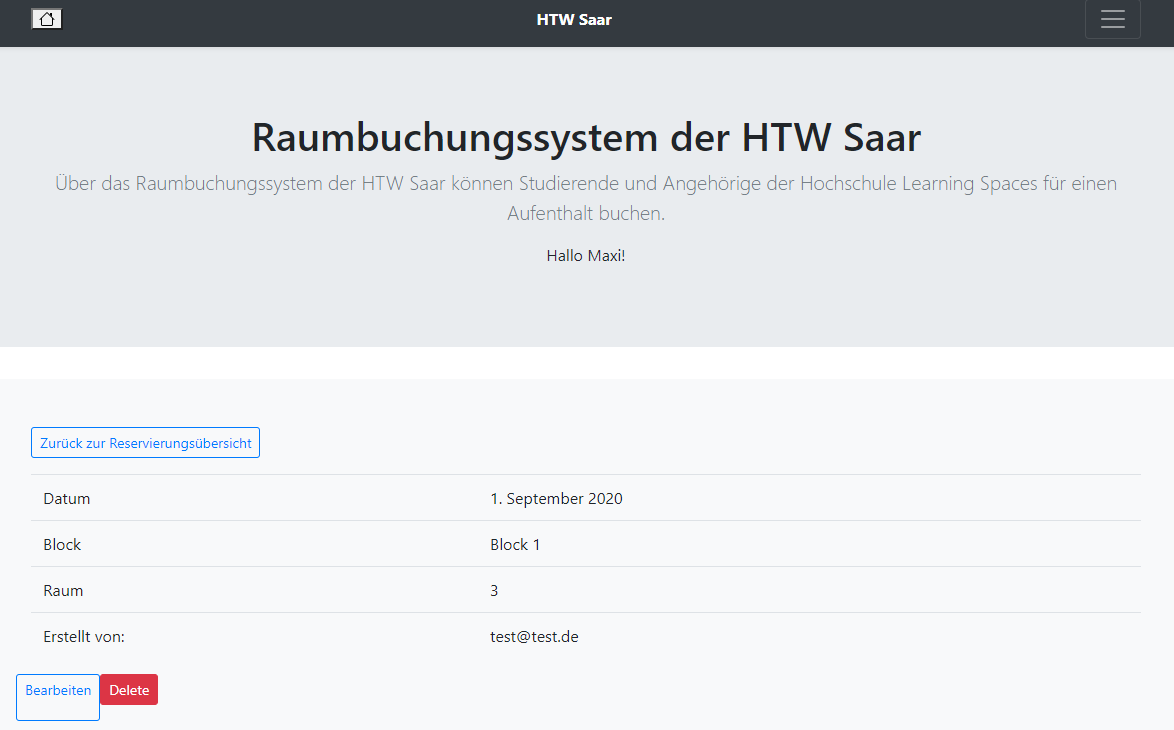
\includegraphics[width=0.8\textwidth]{Stornieren}
    \label{fig:Stornieren}
\end{figure}
Dabei wird vom System eine automatische E-Mail, die die erfolgreiche Stornierung bestätigt, an den User gesendet (L13).
Die Buchung eines Blocks ist maximal sieben Tage im Voraus möglich und jeder User kann in diesem Zeitraum nur maximal einen Block für die geplante Nutzung reservieren. Bei einem weiteren Buchungsversuch wird er darüber informiert, dass ein gebuchter Termin noch aussteht und die gewollte Buchung erst nach Stornierung oder Wahrnehmung möglich ist.
\begin{figure}[h]
    \centering
    \caption{Buchungsinformation}
    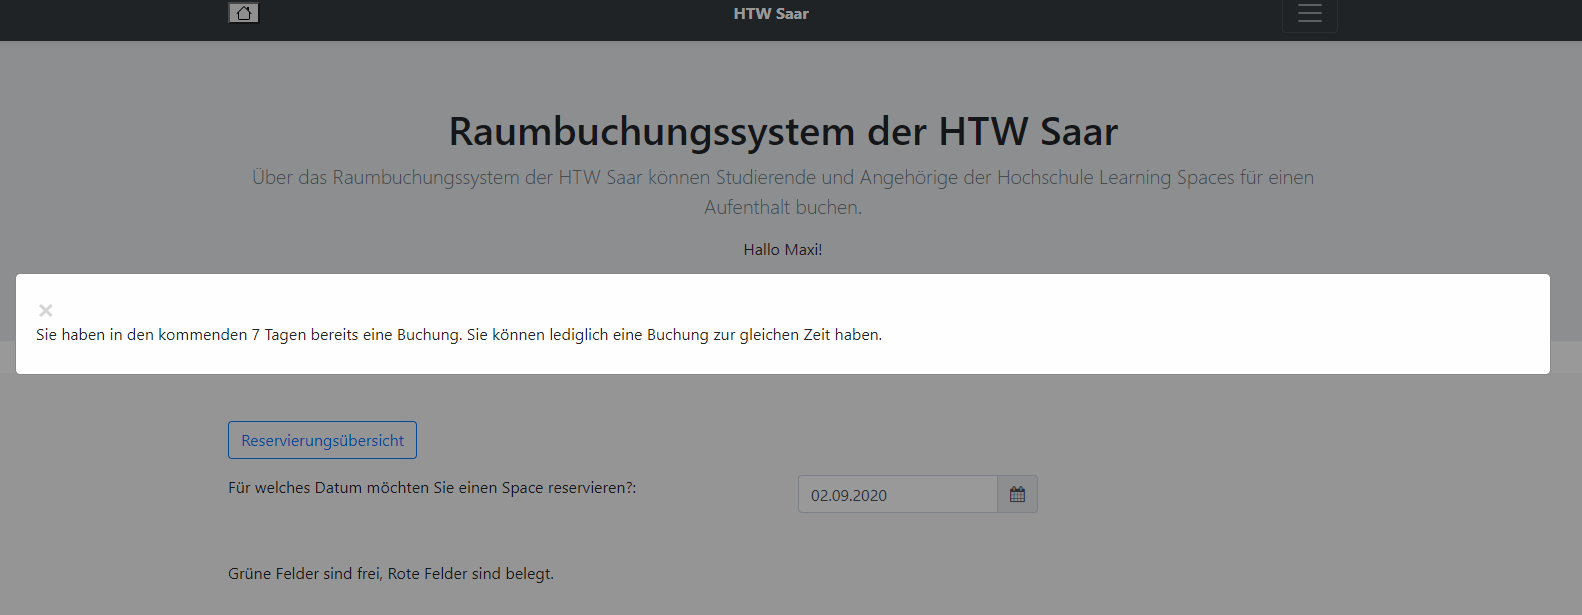
\includegraphics[width=0.8\textwidth]{Buchungsinformation}
    \label{fig:Buchungsinformation}
\end{figure}
\clearpage
Jeder User kann sich seine personenbezogenen Daten, die bei der Erstellung des Nutzerkontos benötigt werden (D10) anzeigen lassen (F23). Weiterhin ist es für den User selbst möglich, das Passwort sowie die E-Mail-Adresse zu ändern und diese Änderung über den „Update“-Button zu aktualisieren (F24).
\begin{figure}[h]
    \centering
    \caption{Personenbezogene Daten}
    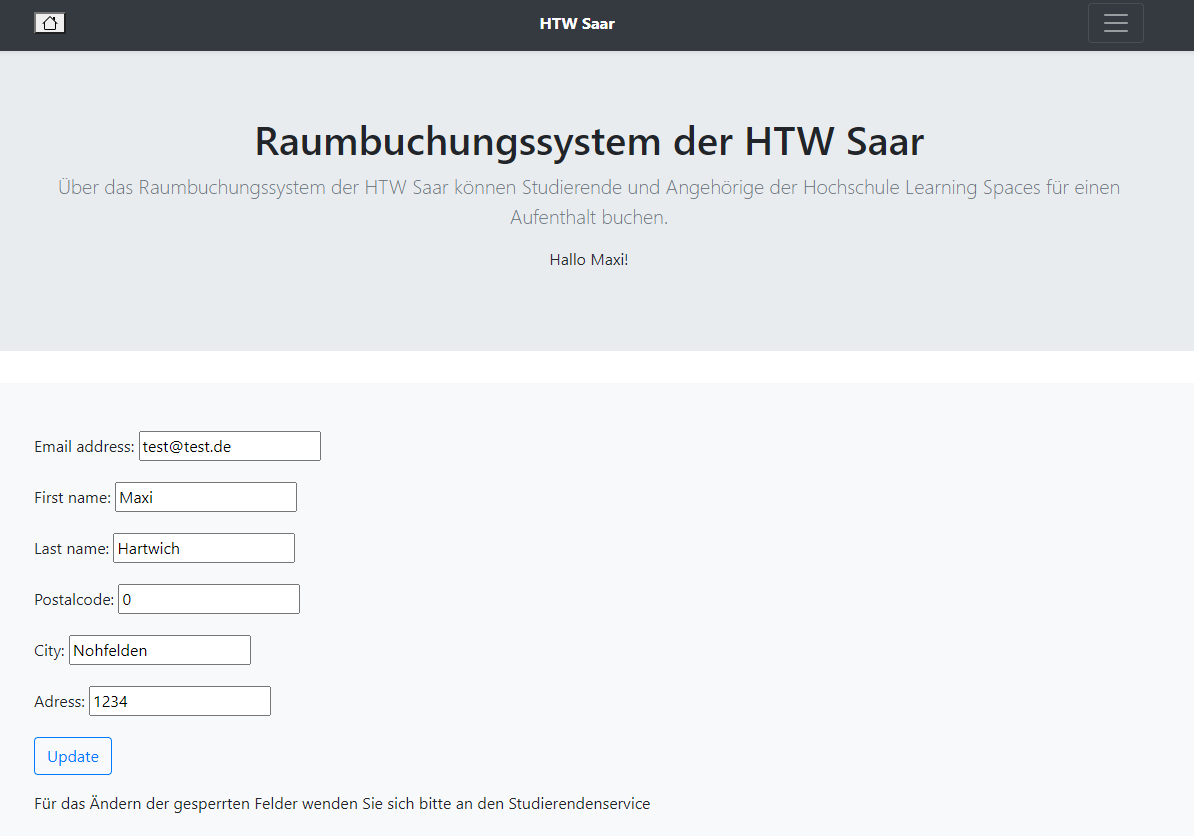
\includegraphics[width=0.8\textwidth]{Personenbezogene Daten}
    \label{fig:Personenbezogene Daten}
\end{figure}

Als Admin des Systems kommen zusätzliche Rechte zu den vorherig genannten hinzu. So kann ein Admin neue Benutzerkonten der drei Usergruppen erstellen (F27) und löschen (F29) und deren zugehörige Daten ändern (F28). Genauso können Daten bezüglich des jeweiligen Learning Spaces angelegt (F30), editiert (F31) oder gelöscht (F32) werden. Die Ressourcen, die jeweils innerhalb eines Learning Spaces angezeigt werden können ebenso vom Admin angelegt (F33), editiert (F34) und gelöscht (F35) werden.
\clearpage
\begin{figure}[h]
    \centering
    \caption{Adminrechte}
    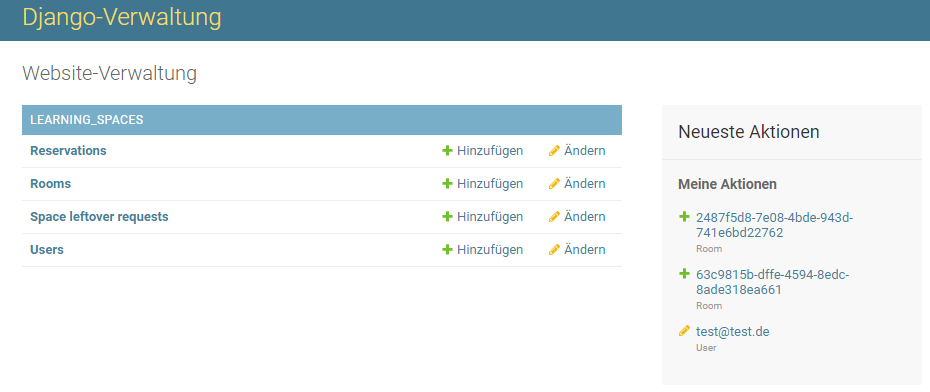
\includegraphics[width=0.8\textwidth]{Adminrechte}
    \label{fig:Adminrechte}
\end{figure}
Der Logout ist jederzeit über den in der Kopfzeile befindlichen Button möglich (F26).\\ \\
\underline{{\large Sonstige Leistungen:}}
\begin{itemize}

\item Fehlermeldung bei falscher Eingabe des Benutzernamens oder Passworts (L10)\\
\item Automatische E-Mail zur Benachrichtigung bei erfolgreicher Buchung (L11)\\
\item Automatische E-Mail zur Benachrichtigung bei erfolgreicher Stornierung der Buchung eines Learning Spaces (L13)
\end{itemize}
\section{Implementierte Kann-Kriterien}

\begin{itemize}
\item \textbf{Mitarbeiter, Dozenten und Studenten der htw saar}
\begin{itemize}
\item Anzeige der Ressourcen in jedem Raum (Plätze, Flipchart oder ähnliches)
\item Hilfe über Kontaktformular anfragen
\end{itemize}

\item Benachrichtigungsemail bei Buchung, Stornierung
\item Dozenten besitzen die Fähigkeit Buchungen zu überschreiben
\item Studenten können anonym belegte Räume anfragen
\item Kontaktaufnahme bei Nachfragen und Komplikationen über Kontaktformular
\item Internationalisierung, sodass das System in englischer Sprache angezeigt und genutzt werden kann
\end{itemize}

\section{Abgrenzungskriterien}\label{abgrenzungskriterien}
\begin{itemize}
\item \textbf{Mitarbeiter, Dozenten und Studenten der htw saar}
\begin{itemize}
\item Admin-Rechte 
\item Vollzugriff auf Daten und Funktionen
\item Mehrfache Raumbuchungen pro Woche 
\item Doppelbelegung eines Spaces durch zwei oder mehrere User
\item Space für länger als einen Zeitblock buchen
\item Buchungen maximal eine Woche im Voraus 
\end{itemize}

\item \textbf{Spaces inklusive externer Displays}
\begin{itemize}
\item Anzeige einzelner Nutzerdaten
\item Anzeige einzelner Admin Funktionen
\end{itemize}
\end{itemize}
\chapter{Beschreibung der durchgeführten Tests}
Durchgeführte Tests siehe in Scrum-Meeting 9 und 10, sowie der vorangegangenen Produktdokumentation.
\chapter{Beschreibung der API Endpunkte}  
Die Beschreibung der API Endpunkte wurde per Software erstellt und ist in einem Browser aufrufbar. Durch diese Art der Darstellung ist es für den Kunden möglich, die API Anfragen in seiner jeweilig gewünschten Sprache angezeigt zu bekommen und Beispielantworten des Servers direkt einzusehen.\\
https://documenter.getpostman.com/view/12423629/TVCcXouz      

\end{document}
